\begin{exercise}{Übung 8.1}
    Man schreibe an jeden Punkt die Koordinaten eines Punktes von $\mathbb{F}^3_2$,
    der die zugehörige Gerade erzeugt. Wieviele verschiedene Lösungen hat diese
    Aufgabe?
\end{exercise}
    \begin{center}
    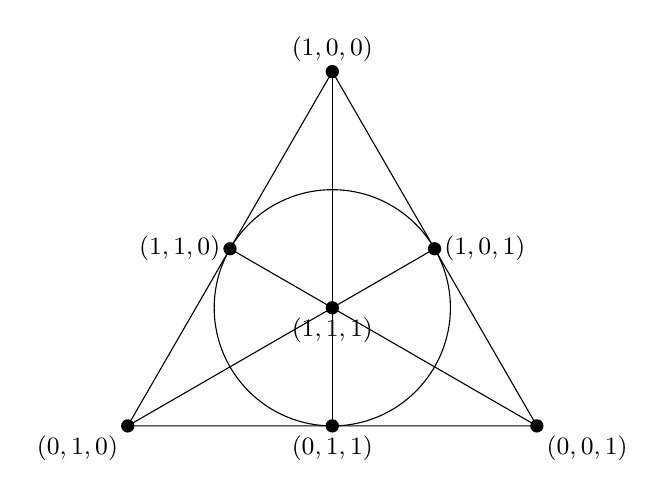
\begin{tikzpicture}[scale=3, every node/.style={font=\small}]
        % Punkte
        \coordinate (A) at (0,1);
        \coordinate (B) at (-0.866,-0.5);
        \coordinate (C) at (0.866,-0.5);

        \coordinate (D) at (-0.433,0.25);
        \coordinate (E) at (0.433,0.25);
        \coordinate (F) at (0,-0.5);

        \coordinate (G) at (0,0);

        % Geraden
        \draw (A) -- (B) -- (C) -- cycle;   % Dreiecksseiten
        \draw (A) -- (F);                    % Gerade A-F-G
        \draw (B) -- (E);                    % Gerade B-E-G
        \draw (C) -- (D);                    % Gerade C-D-G

        % "Kreisgerade" durch D,E,F
        \draw (0,0) circle [radius=0.5];

        % Punkte einzeichnen
        \fill (A) circle (0.8pt) node[above] {$(1,0,0)$};
        \fill (B) circle (0.8pt) node[below left] {$(0,1,0)$};
        \fill (C) circle (0.8pt) node[below right] {$(0,0,1)$};

        \fill (D) circle (0.8pt) node[left] {$(1,1,0)$};
        \fill (E) circle (0.8pt) node[right] {$(1,0,1)$};
        \fill (F) circle (0.8pt) node[below] {$(0,1,1)$};

        \fill (G) circle (0.8pt) node[below] {$(1,1,1)$};
    \end{tikzpicture}
    \end{center}
    Es gibt $7$ von $(0,0,0)$ verschiedene Vektoren in $\mathbb{F}^3_2$.
    Wähle in der Zeichnung drei nicht-kollineare Punkte. Nun benötigen wir drei
    linear unabhängige Vektoren. Für den ersten Punkt gibt es $2^3-1 = 7$ Möglichkeiten.
    Für den zweiten Punkt gibt es $7-1 = 6$ Möglichkeiten. Der dritte Punkt darf
    nicht durch die ersten beiden Punkte erzeugt werden. Daher gibt es für diesen $7-2-1=4$
    Möglichkeiten. Somit gibt es insgesamt
    \[
    \boxed{7 \cdot 6 \cdot 4 = 168 \text{ Lösungen.}}
    \]
\begin{exercise}{Übung 8.2}
    Kann man das Kartenspiel Dobble aus Beispiel 1.5.10,
    ohne neue Symbole hinzuzunehmen, noch um weitere Karten mit acht Symbolen
    ergänzen, so dass immer noch je zwei Karten genau ein Symbol gemeinsam haben?
    Kann man ein verbessertes Dobble konstruieren mit denselben Symbolen, aber
    mehr Karten und denselben Eigenschaften (acht Symbole auf jeder Karte, je zwei
    Karten haben genau ein Symbol gemeinsam)?
\end{exercise}
\textit{Behauptung: } Mit der selben Anzahl an Symbolen kann es höchsten \(57\) Karten geben, sodass die Spieleigenschaften nicht verletzt werden.
\begin{proof}
Wir interpretieren das Kartenspiel wie in Beispiel 1.5.10 als projektive
Ebene
\[
\mathbb P^2\mathbb F_7.
\]
Die Symbole sind die Punkte der projektiven Ebene, die Karten sind die
projektiven Geraden.

Nach Proposition 1.5.6 schneiden sich je zwei verschiedene projektive
Geraden in genau einem Punkt. Daher haben je zwei verschiedene Karten genau
ein gemeinsames Symbol.

Wir zeigen nun, dass man mit denselben Symbolen keine weitere Karte mit
acht Symbolen hinzufügen kann. Dafür benutzen wir nur die folgende Eigenschaft: Es gibt insgesamt $\frac{7^3-1}{7-1}=57$ Symbole, jede Karte
hat \(8\) Symbole, und je zwei verschiedene Karten haben genau ein Symbol
gemeinsam.

Sei nun \(S\) die Menge aller Symbole, \(K_0\subset S\) eine feste Karte und \(s\in K_0\) ein festes Symbol.
Betrachte alle weiteren Karten \(K\neq K_0\), die ebenfalls \(s\) enthalten. Da \(K\) und
\(K_0\) genau ein gemeinsames Symbol haben dürfen, nämlich \(s\), kann
\(K\) kein weiteres Symbol aus \(K_0\) enthalten. Also enthält jede solche
Karte au\ss er \(s\) noch genau \(7\) Symbole aus \(S\setminus K_0\).

Sind \(K\) und \(L\) zwei verschiedene solche Karten mit $s\in K\cap L,$
so dürfen sie au\ss erhalb von \(s\) kein weiteres Symbol gemeinsam haben. Daher sind die Mengen $K\setminus\{s\}$
für diese Karten paarweise disjunkte \(7\)-elementige Teilmengen von
\(S\setminus K_0\).

Da $|S\setminus K_0|=49$, kann es für ein festes \(s\in K_0\) höchstens $\frac{49}{7}=7$ weitere Karten geben, die \(s\) enthalten.

Die Karte \(K_0\) enthält \(8\) Symbole. Jede weitere Karte muss mit
\(K_0\) genau ein Symbol gemeinsam haben. Für jedes dieser \(8\) Symbole gibt es höchstens
\(7\) weitere Karten. Insgesamt gibt es daher höchstens $8\cdot 7=56$ weitere Karten au\ss er \(K_0\).
Zusammen mit \(K_0\) gibt es also höchstens $56+1=57$ Karten.
\end{proof}
\begin{exercise}{Übung 8.3}
Welche Abbildung ist die Zentralprojektion mit Zentrum in $(0, 0, 1) \in \mathbb{R}^3$
auf die $xy$-Ebene in Koordinaten?
\end{exercise}
Sei
\[
N=(0,0,1)
\]
das Zentrum der Zentralprojektion und sei
\[
P=(x,y,z)\in \mathbb R^3
\]
ein Punkt mit \(z\neq 1\).
Die Gerade durch \(N\) und \(P\) ist gegeben durch
\[
N+t(P-N),
\qquad t\in\mathbb R.
\]
Also ist 
\begin{align*}
    N+t(P-N)
    &=
    (0,0,1)+t(x,y,z-1)\\
    &=
    (tx,ty,1+t(z-1)).
\end{align*}
Wir suchen den Schnittpunkt dieser Geraden mit der \(xy\)-Ebene. Diese ist
durch $z=0$ gegeben. Also können wir folgern:
\begin{align*}
    &\phantom{\Leftrightarrow} \quad 1+t(z-1)=0\\
    &\Leftrightarrow \quad t(z-1)=-1\\
    &\Leftrightarrow \quad t=\frac{-1}{z-1} = \frac{1}{1-z}.
\end{align*}
Setzen wir diesen Wert von \(t\) in die Gerade ein, so erhalten wir
\[
(tx,ty,0)
=
\left(
\frac{x}{1-z},
\frac{y}{1-z},
0
\right).
\]
Die Zentralprojektion mit Zentrum \((0,0,1)\) auf die \(xy\)-Ebene ist also
\[
\boxed{
\pi(x,y,z)
=
\left(
\frac{x}{1-z},
\frac{y}{1-z},
0
\right)
\quad \text{für \(z\neq 1\).}
}
\]
\begin{exercise}{Übung 8.4}
    Man zeige, dass die Zentralprojektion mit Zentrum in $(0, 0, 1)$ auf die
    $xy$-Ebene Kreise auf der Einheitssphäre, die $(0, 0, 1)$ nicht enthalten, zu Kreisen
    in der $xy$-Ebene macht. Hinweis: Möbiustransformationen im $\mathbb{R}^3$.
\end{exercise}
\begin{proof}
    Sei
    \[
    N=(0,0,1)
    \]
    und sei
    \[
    S^2=\{(x,y,z)\in\mathbb R^3\mid x^2+y^2+z^2=1\}
    \]
    die Einheitssphäre.
    Wir betrachten die Inversion an der Sphäre mit Zentrum $N$ und Radius
    $\sqrt 2$:
    \[
    \sigma(P)
    =
    N+\frac{2}{\|P-N\|^2}(P-N).
    \]
    Für $P=(x,y,z)\in S^2\setminus\{N\}$ gilt
     \[
    x^2+y^2+z^2=1.
    \]
    Also folgt
    \begin{align*}
        \|P-N\|^2
        &=
        x^2+y^2+(z-1)^2\\
        &=
        x^2+y^2+z^2-2z+1\\
        &=
        2-2z\\
        &=
        2(1-z).
    \end{align*}
    Damit erhalten wir
    \[
    \sigma(x,y,z)
    =
    (0,0,1)+\frac{2}{2(1-z)}(x,y,z-1).
    \]
    Also
    \[
    \sigma(x,y,z)
    =
    \left(
    \frac{x}{1-z},
    \frac{y}{1-z},
    0
    \right).
    \]
    Dies ist genau die Zentralprojektion mit Zentrum $N$ auf die $xy$-Ebene aus Übung 8.3.\\
    Sei nun $C$ ein Kreis auf der Einheitssphäre, der $N$ nicht enthält. Dann
    gibt es eine affine Ebene $E\subset\mathbb R^3$ mit
    \[
    C=S^2\cap E.
    \]
    Da $N\in S^2$ gilt und $N\notin C$, folgt
    \[
    N\notin E.
    \]
    Nach Übung 6.2 wird jede verallgemeinerte
    Sphäre wieder auf eine verallgemeinerte Sphäre abgebildet.
    Da $N \in S^2$, wird
    $S^2$ unter $\sigma$ auf eine erweiterte Ebene abgebildet. Mit Übung 8.3 folgt also
    \[
    \sigma(S^2)=\widehat{\{z=0\}}.
    \]
    Weiter ist $\widehat E=E\sqcup\{\infty\}$ eine erweiterte Ebene, die das
    Inversionszentrum $N$ nicht enthält. Daher ist $\sigma(\widehat E)$
    eine echte Sphäre.\\
    Da $\sigma$ bijektiv ist, gilt
    \[
    \sigma(C)
    =
    \sigma(S^2\cap \widehat E)
    =
    \sigma(S^2)\cap \sigma(\widehat E).
    \]
    Also ist
    \[
    \sigma(C)
    =
    \widehat{\{z=0\}}\cap \sigma(\widehat E).
    \]
    Dies ist der Schnitt der $xy$-Ebene mit einer echten Sphäre, also ein Kreis
    in der $xy$-Ebene.
    Da $\sigma$ auf $S^2\setminus\{N\}$ mit der Zentralprojektion übereinstimmt,
    bildet die Zentralprojektion jeden Kreis auf der Einheitssphäre, der $N$
    nicht enthält, auf einen Kreis in der $xy$-Ebene ab.
\end{proof}